This tutorial presents \textit{testing\_robots}, a simple project to test each robot component one by one. The main goal of this tutorial is for you to compile an mbed project and to understand how to use each sensor.
For some sensors, you'll have to develop the function accessing the data. For others, everything is already done and the program uses the provided library.



\begin{UPSTIactivite}[][Import the project][][][To do]

 \begin{enumerate}
  \item Using $\vcenter{\hbox{
\includegraphics[height=2\fontcharht\font`\B]{images/firefox}}}$ \textbf{Firefox}, go on the mbed website : \url{https://www.mbed.com/en/} and log in or create an account.
  \item Visit \url{https://os.mbed.com/users/gvaquette/code/workshop_tutorial/}
  \item Add the project to your compiler : $\vcenter{\hbox{ 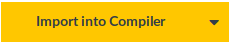
\includegraphics[height=3\fontcharht\font`\B]{images/import_compiler}}}$
 \end{enumerate}


\end{UPSTIactivite}

Import it into your mbed compiler before continuing.
Here the project tree :

\dirtree{%
 .0 /.
 .1 lib\_workshop\_2019 \DTcomment{Provided library to run the robot}.
 .2 CMPS03 \DTcomment{Compass library}.
 .2 CNY70  \DTcomment{Library for reflective sensors}.
 .2 PID    \DTcomment{Library for PID}.
 .2 Pixy   \DTcomment{Library for Pixy camera}.
 .2 VMA306 \DTcomment{Library for ultrasonic sensors}.
 .1 includes.
 .2 console\_output.h.
 .2 pin\_connexions.h \DTcomment{Declare and connect signals}.
 .2 test\_cny.h.
 .2 test\_compass.h.
 .2 test\_motor.h.
 .2 test\_us.h \DTcomment{for ultrasonic sensors}.
 .1 src.
 .2 test\_cny \DTcomment{function files to use cny70 sensors}.
 .2 test\_compass \DTcomment{function files to use compass sensor}.
 .2 test\_motor \DTcomment{function files to run motors}.
 .2 test\_us \DTcomment{function files to use ultrasonic sensors}.
 .2 console\_output.cpp \DTcomment{function to print messages to pc.}.
 .1 main.cpp.
}

The main file run an infinite loop asking the user which test does he want to run and calling the associated function.
